\documentclass[12pt]{eskdtext}
\usepackage[numbertop, numbercenter]{eskdplain}
\usepackage[utf8x]{inputenc}

% - Подключаем шрифты из пакета scalable-cyrfonts-tex
\usepackage{cyrtimes}

% - Отступ красной строки
\setlength{\parindent}{1.25cm}

% - Убирает точку в списке литературы
\makeatletter
\def\@biblabel#1{#1 }

% - Точки для всех пунктов в оглавлении
\renewcommand*{\l@section}{\@dottedtocline{1}{1.5em}{2.3em}}
\renewcommand*{\l@subsection}{\@dottedtocline{1}{1.5em}{2.3em}}
\renewcommand*{\l@subsubsection}{\@dottedtocline{1}{1.5em}{2.3em}}

% - Для переопределения списков
\renewcommand{\theenumi}{\arabic{enumi}}
\renewcommand{\labelenumi}{\theenumi)}
\makeatother

\usepackage{enumitem}
\setlist{nolistsep, itemsep=0.3cm,parsep=0pt}

% - ГОСТ списка литературы
\bibliographystyle{utf8gost705u}

% - Верикальные отступы заголовков 
\ESKDsectSkip{section}{1em}{1em}
\ESKDsectSkip{subsection}{1em}{1em}
\ESKDsectSkip{subsubsection}{1em}{1em}

% - Изменение заголовков
\usepackage{titlesec}
\titleformat{\section}{\centering\normalfont\normalsize}{\thesection}{1.0em}{}
\titleformat{\subsection}{\centering\normalfont\normalsize}{\thesubsection}{1.0em}{}
\titleformat{\subsubsection}{\centering\normalfont\normalsize}{\thesubsubsection}{1.0em}{}
\titleformat{\paragraph}{\centering\normalsize}{\theparagraph}{1.0em}{}

% - Оставим место под ТЗ 
%\setcounter{page}{4}

% - Для больших таблиц
\usepackage{longtable}
\usepackage{tabularx}
\renewcommand{\thetable}{\thesection.\arabic{table}}

% - Используем графику в документе
\usepackage{graphicx}
\graphicspath{{images/}}
\renewcommand{\thefigure}{\thesection.\arabic{figure}}

% - Счётчики
\usepackage{eskdtotal}

% - Выравнивание по ширине
\sloppy

% - Разрешить перенос двух последних букв слова
\righthyphenmin=2

\RequirePackage{enumitem}
\renewcommand{\alph}[1]{\asbuk{#1}}
\setlist{nolistsep}
\setitemize[1]{label=--, fullwidth, itemindent=\parindent, 
  listparindent=\parindent}% для дефисного списка
\setenumerate[1]{label=\arabic*), fullwidth, itemindent=\parindent, 
  listparindent=\parindent}% для нумерованного списка
\setenumerate[2]{label=\alph*), fullwidth, itemindent=\parindent, 
  listparindent=\parindent, leftmargin=\parindent}% для списка 2-ой ступени, который будет нумероваться а), б) и т.д.

% - Оформляем листинг кода (не использовать комментарии на русском!)
\usepackage{listings}  
\lstset{basicstyle=\ttfamily\small}
\lstset{extendedchars=\true}

% - выводим текст как есть с размером шрифта scriptsize
\makeatletter
\def\verbatim{\scriptsize\@verbatim \frenchspacing\@vobeyspaces \@xverbatim}
\makeatother


\begin{document}
 \newpage
\ESKDthisStyle{empty}

\begin{center}
 Министерство образования и науки Российской Федерации\\
 Федеральное государственное бюджетное образовательное учреждение высшего профессионального образования\\
 <<ТОМСКИЙ ГОСУДАРСТВЕННЫЙ УНИВЕРСИТЕТ СИСТЕМ УПРАВЛЕНИЯ И РАДИОЭЛЕКТРОНИКИ>> (ТУСУР)\\
 Кафедра комплексной информационной безопасности электронно-вычислительных систем (КИБЭВС)\\
\end{center}

\vfill

\begin{flushright}
\begin{minipage}{0.45\textwidth}
 \begin{flushleft}
  УТВЕРЖДАЮ\\
  заведующий каф. КИБЭВС
  \underline{\hspace{3cm}}А.А. Шелупанов \\
  <<\underline{\hspace{1cm}}>>\underline{\hspace{3cm}}2016г.\\
 \end{flushleft}
\end{minipage}
\end{flushright}

\vfill

\begin{center}
ПРОГРАММНЫЙ КОМПЛЕКС ДЛЯ ПРОВЕДЕНИЯ СОРЕВНОВАНИЙ В ОБЛАСТИ ИНФОРМАЦИОННОЙ БЕЗОПАСНОСТИ

Отчет по групповому проектному обучению

Группа КИБЭВС-1502
\end{center}

\vfill
\begin{flushright}
\begin{minipage}{0.45\textwidth}
 \begin{flushleft}
  Ответственный исполнитель \\
  студент гр. 723 \\
  \underline{\hspace{3cm}}Д.Е. Муковкин \\
  <<\underline{\hspace{1cm}}>>\underline{\hspace{3cm}}2016г.\\
 \end{flushleft}
\end{minipage}
\end{flushright}

\vfill

\begin{flushright}
\begin{minipage}{0.45\textwidth}
 \begin{flushleft}
  Научный руководитель \\
  аспирант каф. КИБЭВС \\
  \underline{\hspace{3cm}}А.И. Гуляев \\
  <<\underline{\hspace{1cm}}>>\underline{\hspace{3cm}}2016г.\\
 \end{flushleft}
\end{minipage}
\end{flushright}

\vfill

\begin{center}
 2016
\end{center}

 \newpage
\ESKDthisStyle{empty}
\paragraph{\hfill РЕФЕРАТ \hfill}
Курсовая работа содержит \ESKDtotal{page} страниц, \ESKDtotal{figure} рисунка, \ESKDtotal{table} таблицы, \ESKDtotal{bibitem} источников, \ESKDtotal{appendix} приложение.

%допилить ключевые слова
КОМПЬЮТЕРНАЯ ЭКСПЕРТИЗА, ФОРЕНЗИКА, ЛОГИ, QT, XML, GIT, LATEX, MOZILLA THUNDERBIRD, MS OUTLOOK, WINDOWS, PST, MSG, RTF, HTML, БИБЛИОТЕКИ, РЕПОЗИТОРИЙ, ПОЧТОВЫЙ КЛИЕНТ, SQLLITE, РЕЕСТР, МЕТА-ДАННЫЕ, READPST, JPEG, PNG, ID3V1, JFIF, RIFF, CHUNK, DBX, C++, DOXYGEN.

Цель работы --- создание программного комплекса, предназначенного для проведения компьютерной экспертизы.

Задачей, поставленной на данный семестр, стало написание программного комплекса, имеющего следующие возможности: 
\begin{enumerate}
\item сбор и анализ информации из журналов истории браузеров;
\item сбор и анализ информации из мессенджеров;
\item сбор и анализ информации из почтовых приложений;
\item поиск медиа-файлов (аудио, видео, изображение) и извлечение мета-данных из них;
\item сбора информации об установленном ПО по остаточным файлам.
\item сбор и анализ информации из реестра Windows.
\end{enumerate}

Результаты работы в данном семестре:

\begin{itemize}
\item реализован импорт истории посещений, поисковых запросов, загруженных файлов, списка установленных расширений, информации о версии программы и подключенном аккаунтеGoogle из приложения Google Chrome;
\item реализован алгоритм сканирования директорий ОС Windows на содержание файлов, оставшихся при установке или после удаления различных программ;
\item реализован алгоритм извлечения адресата, отправителя, темы, даты и текста
сообщения из файлов формата <<.dbx>>, используемого MS Outlook для хранения сообщений;
\item реализован алгоритм извлечения времени, даты, отправителя, получателя и текст
сообщения почтового клиента Mozilla Thunderbird;
\item реализован алгоритм извлечения мета-данных из фалов формата ID3v1, JFIF и RIFF;
\item реализован алгоритм извлечения информации из реестра Windows (.reg-файлов).
\end{itemize}

Пояснительная записка выполнена при помощи системы компьютерной вёрстки \LaTeX.

 
 \newpage
 \ESKDthisStyle{empty}
 \section*{Список исполнителей}

Муковкин Д.Е. -- программист, ответственный исполнитель.

Задачи:
\begin{itemize}
\item выбор языка программирования;
\item создание архитектуры ядра;
\item развертывание инфраструктуры;
\item разработка модуля проверки сервисов, сдача флагов;
\item настройка и тестирование платформы.
\end{itemize}

Койшинов Т.С. -- программист.

Задачи:
\begin{itemize}
\item разработка структуры БД в API;
\item доработка панели администратора;
\item разработка API функций;
\item разработка модуля таблицы результатов.
\end{itemize}
 
 % - содержание
 \newpage
 \ESKDstyle{plain}
 \tableofcontents

 \newpage
 \ESKDstyle{plain}
 \section*{Введение}
 \addcontentsline{toc}{section}{Введение}
 CTF (Capture the flag, Захват флага) - это командные соревнования, целью которых является оценка умения участников атаковать и защищать компьютерные системы. По типу, соревнования делятся на два типа: task-based (квесты), attack-defense (классические соревнования).

Для проведения соревнований типа attack-defense, каждой команде выдается сервер, на котором имеется ряд сервисов, одинаковые у всех. Сервисами являются программы, которые должны быть запущены на протяжении всего времени соревнований. Раз в минуту жюрейская система проверяет работу сервисов, присылает новый флаг, а также проверяет его наличие на сервере. В роли флага выступает случайно сгенерированная строка, определенной длины. Сервисы заведомо имеют уязвимости, через которые можно украсть флаг. Команда должна найти уязвимости в сервисах и закрыть их. Но также она должна эксплуатировать эти уязвимости на сервисах других команд, похищая флаги. 

Команда Keva имеет большой опыт в проведении соревнований CTF. Во время проведения межрегиональных межвузовских соревнований в области информационной безопасности SibirCTF 2014, 2015 использовались наработки Екатеринбургской команды HackerDom. Однако их решение не подходит нам по некоторым критически важным параметрам. Поэтому  было принято решение написать собственную платформу для проведения соревнований CTF.

Платформа должна отвечать следующим требованиям:
\begin{itemize}
\item Низкое потребление ресурсов сервера;
\item Управление игрой через графический интерфейс;
\item Возможность горизонтального масштабирования.
\end{itemize}

При разработке платформы должны быть использованы уже имеющиеся наработки, в частности, панель администратора и API для task-based проведения соревнований. 

Новая платформа позволит проводить собственные соревнования не используя готовые решения. 

 \newpage
 \section{Назначение и область применения}
Разрабатываемый программно-аппаратный комплекс предназначен для проведения игр в области информационной безопасности Capture the flag по типу Attack-Defense.
\section{Постановка задачи}
\setcounter{figure}{0}
В данной курсовой работе были поставлены следующие задачи:

\begin{itemize}
\item выбор инструментов разработки платформы;
\item разработка архитектуры;
\item определение индивидуальных задач для каждого участника проектной группы;
\item исследование предметных областей в рамках индивидуальных задач;
\item реализация новых программных модулей и доработка уже существующих.
\end{itemize}

Задачи, связанные с разработкой программного комплекса:

\begin{enumerate}
\item разработка ядра платформы;
\item разработка модуля проверяющей системы;
\item разработка модуля сдачи флага;
\item разработка модуля рейтинговой таблицы;
\item доработка модуля администраторской панели.
\end{enumerate}

Задачи, связанные с тестированием программного комплекса:

\begin{enumerate}
\item проверка работы ядра;
\item проверка работы модуля проверяющей системы;
\item проверка работы модуля сдачи флага;
\item проверка работы модуля рейтинговой таблицы;
\item проверка работы модуля администраторской панели.
\end{enumerate}

\section{Инструменты}
\setcounter{figure}{0}
\subsection{Система контроля версий Git}
Для разработки программного комплекса для проведения компьютерной экспертизы было решено использовать Git.

Git --- распределённая система управления версиями файлов. Проект был создан Линусом Торвальдсом для управления разработкой ядра Linux  как противоположность  системе управления версиями Subversion (также известная как «SVN») \cite{progit}.

При работе над одним проектом команде разработчикоа необходим инструмент для совместного написания, бэкапирования и тестирования программного обеспечения. Используя Git, мы имеем:
\begin{itemize}
\item возможность удаленной работы с исходными кодами;
\item возможность создавать свои ветки, не мешая при этом другим разработчикам;
\item доступ к последним изменениям в коде, т.к. все исходники хранятся на сервере git.keva.su;
\item исходные коды защищены, доступ к ним можно получить лишь имея RSA-ключ;
\item возможность откатиться к любой стабильной стадии проекта.
\end{itemize}

Основные постулаты работы с кодом в системе Git:

\begin{itemize}
\item каждая задача решается в своей ветке;
\item необходимо делать коммит как только был получен осмысленный результат;
\item ветка master мержится не разработчиком, а вторым человеком, который производит вычитку и тестирование изменения;
\item все коммиты должны быть осмысленно подписаны/прокомментированы.
\end{itemize}

Для работы над проектом проектной группой был поднят собственный репозиторий на сервере git.keva.su.
Адреса репозиториев следующие:

Исходные файлы проекта:

git clone git@git.keva.su:gpo.git gpo.git

Репозиторий для тестирования проекта:

git clone git@git.keva.su:gpo-testdata.git gpo-testdata.git

\subsection{Система компьютерной вёрстки \TeX}
\TeX\ --- это созданная американским математиком и программистом Дональдом Кнутом система для вёрстки текстов. Сам по себе \TeX\ представляет собой специализированный язык программирования.Каждая издательская система представляет собой пакет макроопределений этого языка.

\LaTeX\ --- это созданная Лэсли Лэмпортом издательская система на базе \TeX'а\cite{lvovskyi}. \LaTeX\ позволяет пользователю сконцентрировать свои услия на содержании и структуре текста, не заботясь о деталях его оформления.

Для подготовки отчётной и иной документации нами был выбран \LaTeX\, так как совместно с системой контроля версий Git он предоставляет возможность совместного создания и редактирования документов. Огромным достоинством системы \LaTeX\ то, что создаваемые с её помощью файлы обладают высокой степенью переносимости \cite{latexrus}.

Совместно с \LaTeX\ часто используется Bib\TeX\ --- программное обеспечение для создания форматированных списков библиографии. Оно входит в состав дистрибутива \LaTeX\ и позволяет создавать удобную, универсальную и долговечную библиографию. Bib\TeX\ стал одной из причин, по которой нами был выбран \LaTeX\ для создания документации.

\subsection{Язык программирования Python}
Python --- высокоуровневый язык программирования общего назначения, ориентированный на повышение производительности разработчика и читаемости кода. Синтаксис ядра Python минималистичен. В то же время стандартная библиотека включает большой объём полезных функций \cite{python_wiki}. 


Основные архитектурные черты — динамическая типизация, автоматическое управление памятью, полная интроспекция, механизм обработки исключений, поддержка многопоточных вычислений и удобные высокоуровневые структуры данных. Код в Python организовывается в функции и классы, которые могут объединяться в модули.

Основными преимуществами языка программирования Python являются большое количество библиотек, кроссплатформенность, широкие возможности профилирования кода. 

Язык обладает чётким и последовательным синтаксисом, продуманной модульностью и масштабируемостью, благодаря чему исходный код написанных на Python программ легко читаем. При передаче аргументов в функции Python использует вызов по соиспользованию.

Разработка языка Python была начата в конце 1980-х годов сотрудником голландского института CWI Гвидо ван Россумом.
\subsection{База данных MongoDB}
Для реализации программного комплекса для проведения соревнований в области информационной безопасноти была использована база данных MongoDB.

MongoDB --- документо-ориентированная система управления базами данных (СУБД) с открытым исходным кодом, не требующая описания схемы таблиц. Написана на языке C++. \cite{mongo}.

Основные возможности MongoDB:
\begin{itemize}
\item Документо-ориентированное хранение (JSON-подобная схема данных);
\item Достаточно гибкий язык для формирования запросов;
\item Динамические запросы;
\item Поддержка индексов;
\item Профилирование запросов;
\item Быстрые обновления «на месте»;
\item Эффективное хранение двоичных данных больших объёмов, например, фото и видео;
\item Журналирование операций, модифицирующих данные в базе данных;
\item Поддержка отказоустойчивости и масштабируемости: асинхронная репликация, набор реплик и распределения базы данных на узлы;
\item Возможность работы в соответствии с парадигмой MapReduce;
\item Полнотекстовый поиск, в том числе на русском языке, с поддержкой морфологии.
\end{itemize}

Архитектура:

СУБД управляет наборами JSON-подобных документов, хранимых в двоичном виде в формате BSON. Хранение и поиск файлов в MongoDB происходит благодаря вызовам протокола GridFS. Подобно другим документо-ориентированным СУБД (CouchDB и др.), MongoDB не является реляционной СУБД. В СУБД:

\begin{itemize}
\item Нет такого понятия, как «транзакция». Атомарность гарантируется только на уровне целого документа, то есть частичного обновления документа произойти не может;
\item Отсутствует понятие «изоляции». Любые данные, которые считываются одним клиентом, могут параллельно изменяться другим клиентом.
\end{itemize}

В MongoDB реализована асинхронная репликация в конфигурации «ведущий — ведомый» (англ. master — slave), основанная на передаче журнала изменений с ведущего узла на ведомые. Поддерживается автоматическое восстановление в случае выхода из строя ведущего узла. Серверы с запущенным процессом mongod должны образовать кворум, чтобы произошло автоматическое определение нового ведущего узла. Таким образом, если не используется специальный процесс-арбитр (процесс mongod, только участвующий в установке кворума, но не хранящий никаких данных), количество запущенных реплик должно быть нечётным.

\subsection{TrackingTime - Система управления проектами и задачами}

TrackingTime --- это сервис, предоставляющий возможность управлять своими проектами, задачами, персонал.

Основным преимуществом является удобный учет времени ответственного за задачу. 
Проект декомпозируется на этапы и задачи.
Каждая задача назначается на ответственного работника, который в свою очередь при её выполнении устанавливает таймер.

Приложение доступно на всех основных платформах (Windows, Linux, OS X, iOS, Android)
\subsection{Flask - микрофреймворк для Python}
\ESKDthisStyle{empty}
Flask - это микрофреймворк, написанный на языке программирования Python, основанный на Werkzeug и Jinja 2. Выпускается под BSD лицензией.

Слово «микро» означает, что цель написания фреймворка - сохранить ядро простым, но в то же время легко расширяемой. По умолчанию Flask не включает в себя уровень абстракции базы данных, валидацию форм или другие библиотеки, которые с легкостью можно подключить. Вместо этого Flask поддерживает механизм расширения существующего кода так, как будто он уже был подключен к нему. Множество расширений предоставляют интеграцию с базой данных, валидацию форм, поддержку загрузки файлов, аутентификации пользователя и другие полезные функции.

Особенности фреймворка 
\begin{itemize}
\item удобная работа с URL;
\item богатые возможности шаблонизатора;
\item минимальные требования к ресурсам в сравнении с аналогичными фреймворками.
\end{itemize}

Flask используется в модуле таблицы рейтинга. 

\newpage
\section{Технические характеристики}
\subsection {Требования к аппаратному обеспечению}

Необходимо 2 и более компьютера, находящихся в локальной сети.

Минимальные системные требования:

\begin{itemize}
\item процессор 1ГГц Pentium 4;
\item оперативная память 512 Мб;
\item место на жёстком диске -- 9 Гб.
\end{itemize}

\subsection {Требования к программному обеспечению}
Для корректной работы разрабатываемого программного комплекса на компьютере должны быть установлены пакеты: Python 3.X, MongoDB. 


\section{Разработка программного обеспечения}
\setcounter{figure}{0}
 
\subsection{Архитектура}
\subsubsection{Основной алгоритм}
В ходе разарботки был применен видоизменнённый шаблон проектирования Factory method.


\subsection{Модуль: прием и проверка принятых флагов} % - Отчёт flags
В соревнованиях по информационной безопасности задача команд найти уязвимость и эксплуатировать её, добывая секретную информацию, в нашем случае флаги. Целью модуля является прием и проверка на валидность флагов.

\subsubsection{Принцип работы}

Программа реализована с использованием вебсокетов. На порту, полученном с API, программа сравнивает IP адрес клиента с данными в базе данных и при нахождении его, клиент определяется как одна из команд и может отправить серверу строку. Строка проверяется на длину символов. Так же флаг проверяется на наличие в базе данных, времени его жизни (флаги валидны определенное количество времени), принадлежность другой команде (свои флаги сдавать нельзя) и статус сервиса (аналогичный сервис сдающей команды должен быть поднят). 

Ниже представлен алгоритм и наглядная схема работы flags.py

\begin{figure}[h!]
\center{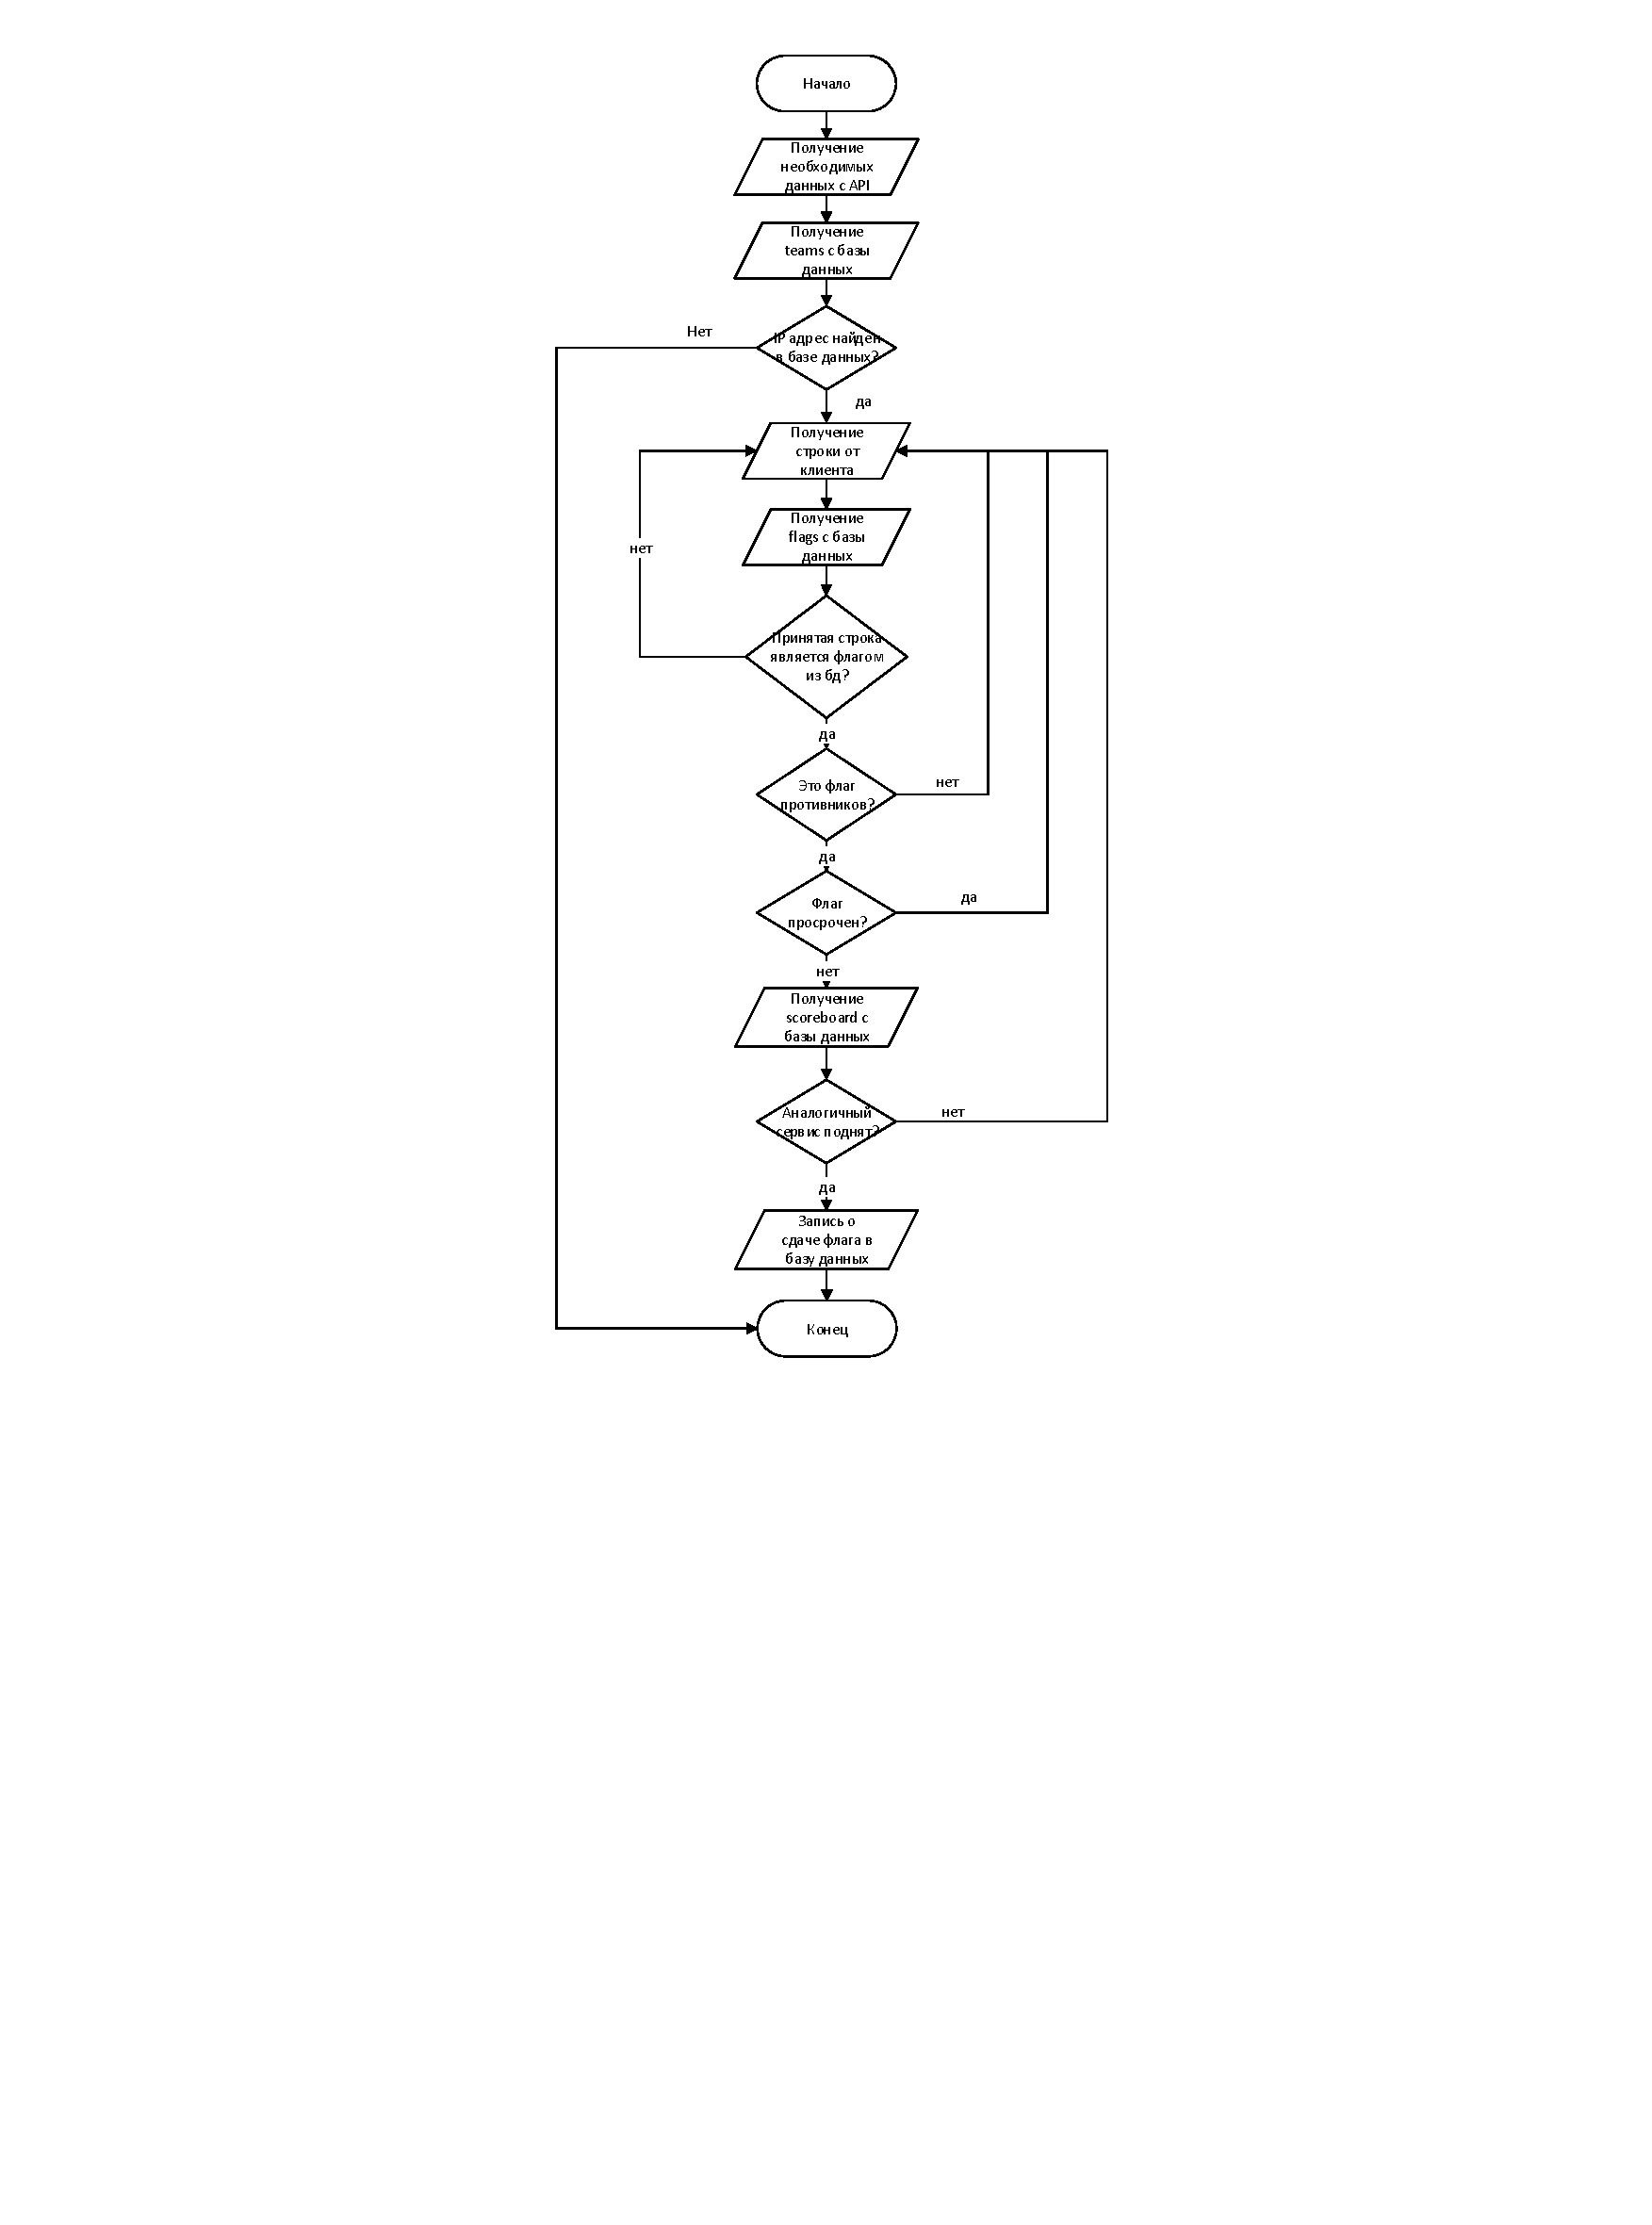
\includegraphics[trim=200 400 200 0, width=0.7\linewidth]{individual_reports/Algoritm.pdf}}
\caption{Алгоритм модуля flags.py}
\end{figure} 

\begin{figure}[h!]
\center{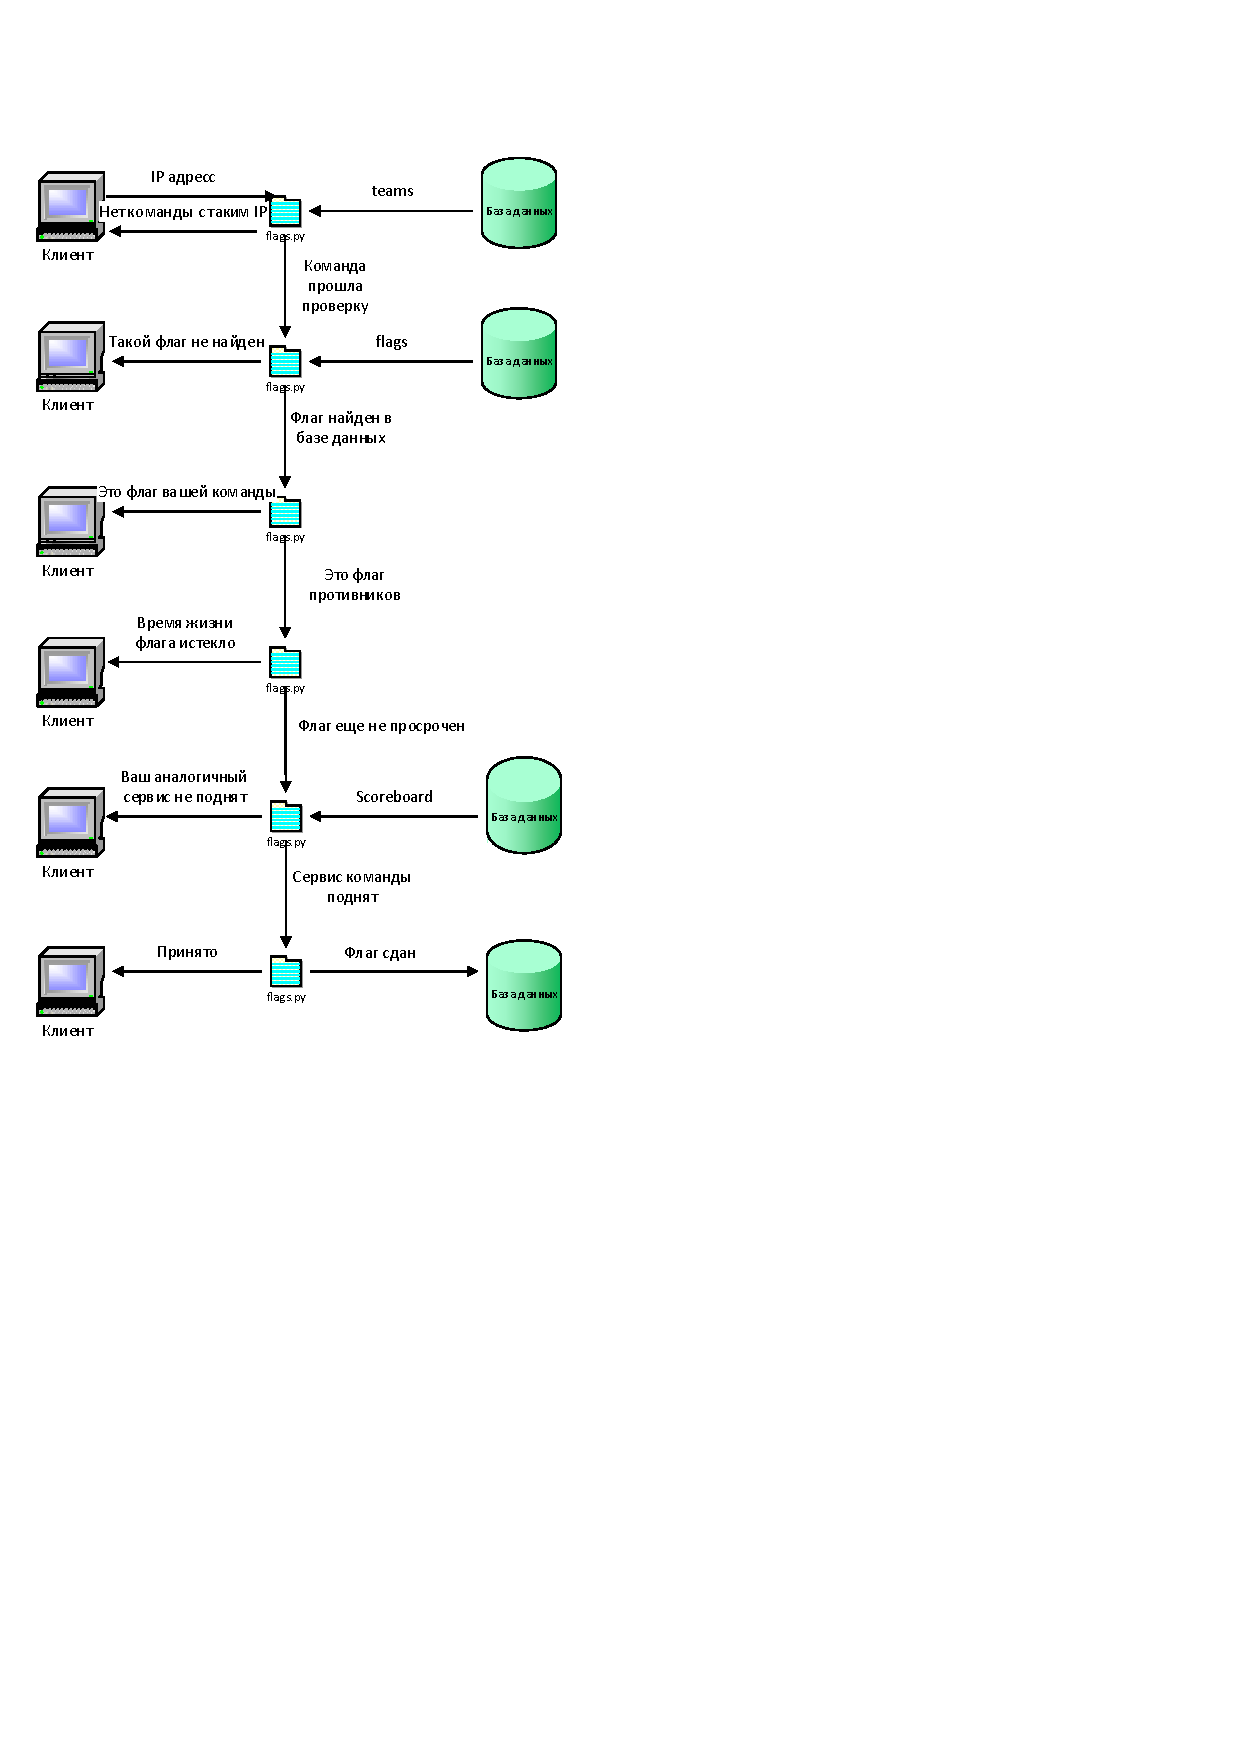
\includegraphics[trim=0 300 300 0, width=0.7\linewidth]{individual_reports/Naglyadno.pdf}}
\caption{Наглядная схема работы flags.py}
\end{figure} 

\clearpage


\subsection{Модуль: таблицы результатов} % - Отчёт scoreboard
В соревнованиях по информационной безопасности задача команд найти уязвимость и эксплуатировать её, добывая секретную информацию, в нашем случае флаги. Целью модуля является прием и проверка на валидность флагов.

\subsubsection{Принцип работы}

Программа реализована с использованием вебсокетов. На порту, полученном с API, программа сравнивает IP адрес клиента с данными в базе данных и при нахождении его, клиент определяется как одна из команд и может отправить серверу строку. Строка проверяется на длину символов. Так же флаг проверяется на наличие в базе данных, времени его жизни (флаги валидны определенное количество времени), принадлежность другой команде (свои флаги сдавать нельзя) и статус сервиса (аналогичный сервис сдающей команды должен быть поднят). 

Ниже представлен алгоритм и наглядная схема работы flags.py

\begin{figure}[h!]
\center{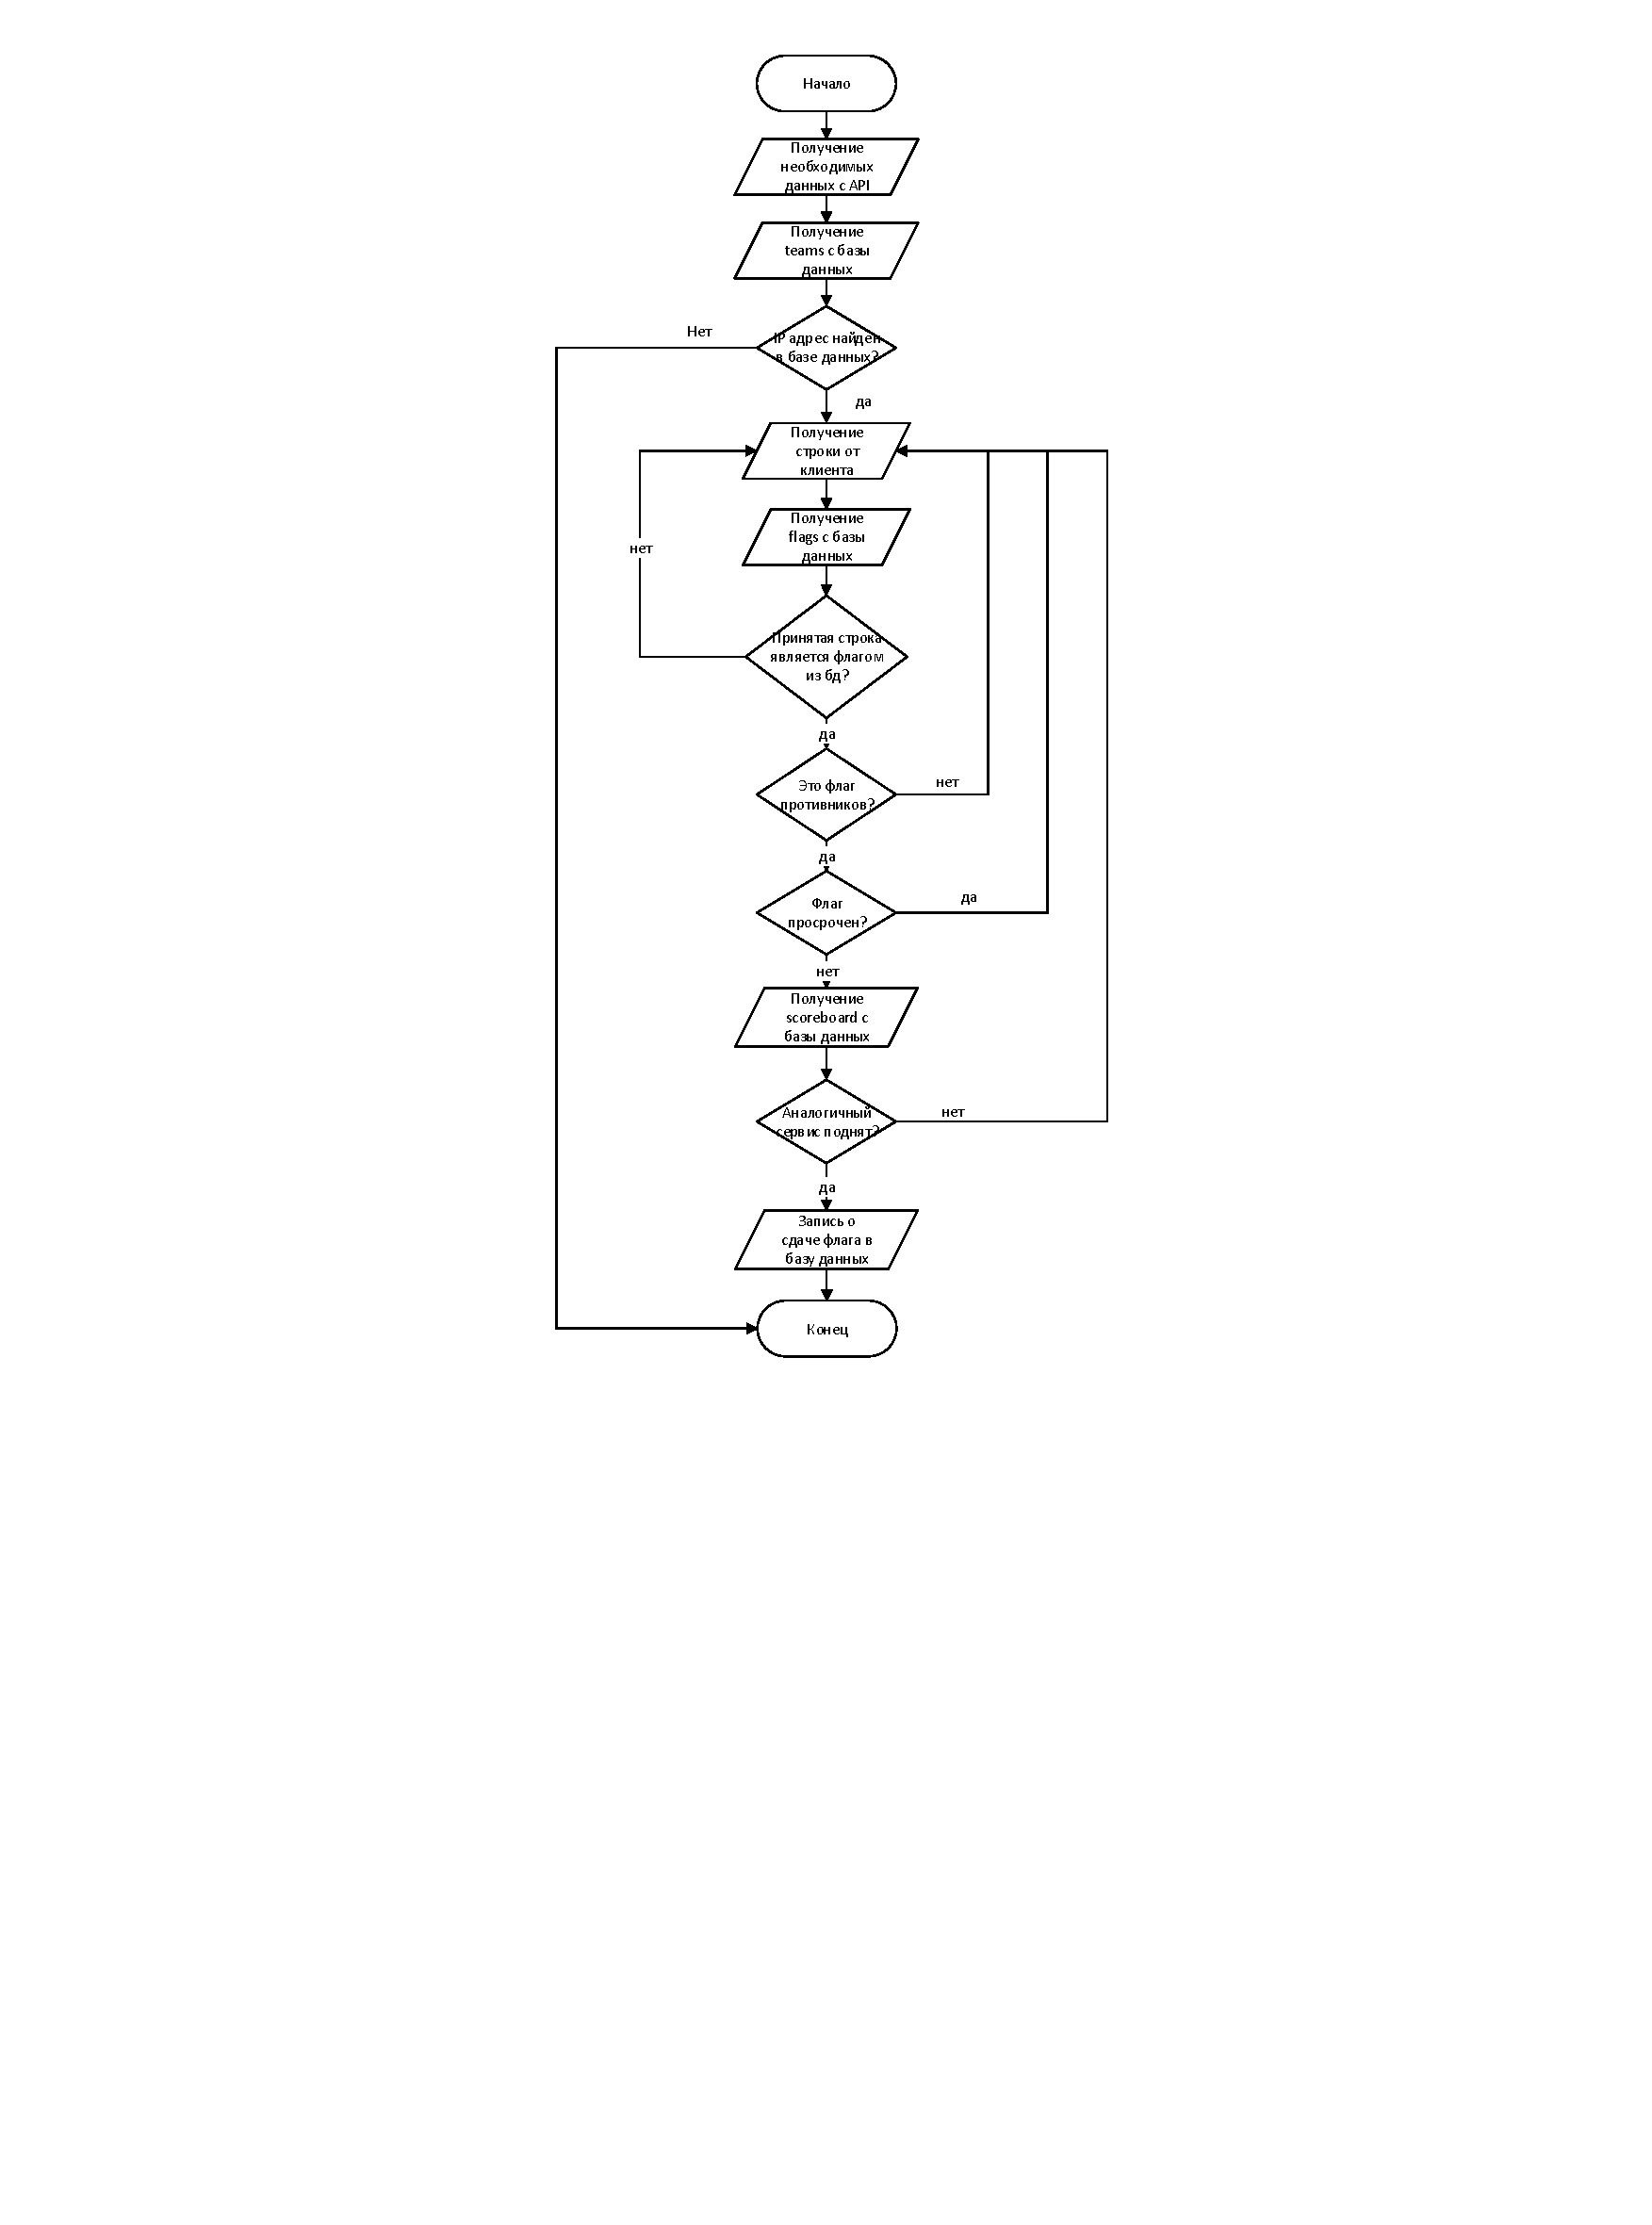
\includegraphics[trim=200 400 200 0, width=0.7\linewidth]{individual_reports/Algoritm.pdf}}
\caption{Алгоритм модуля flags.py}
\end{figure} 

\begin{figure}[h!]
\center{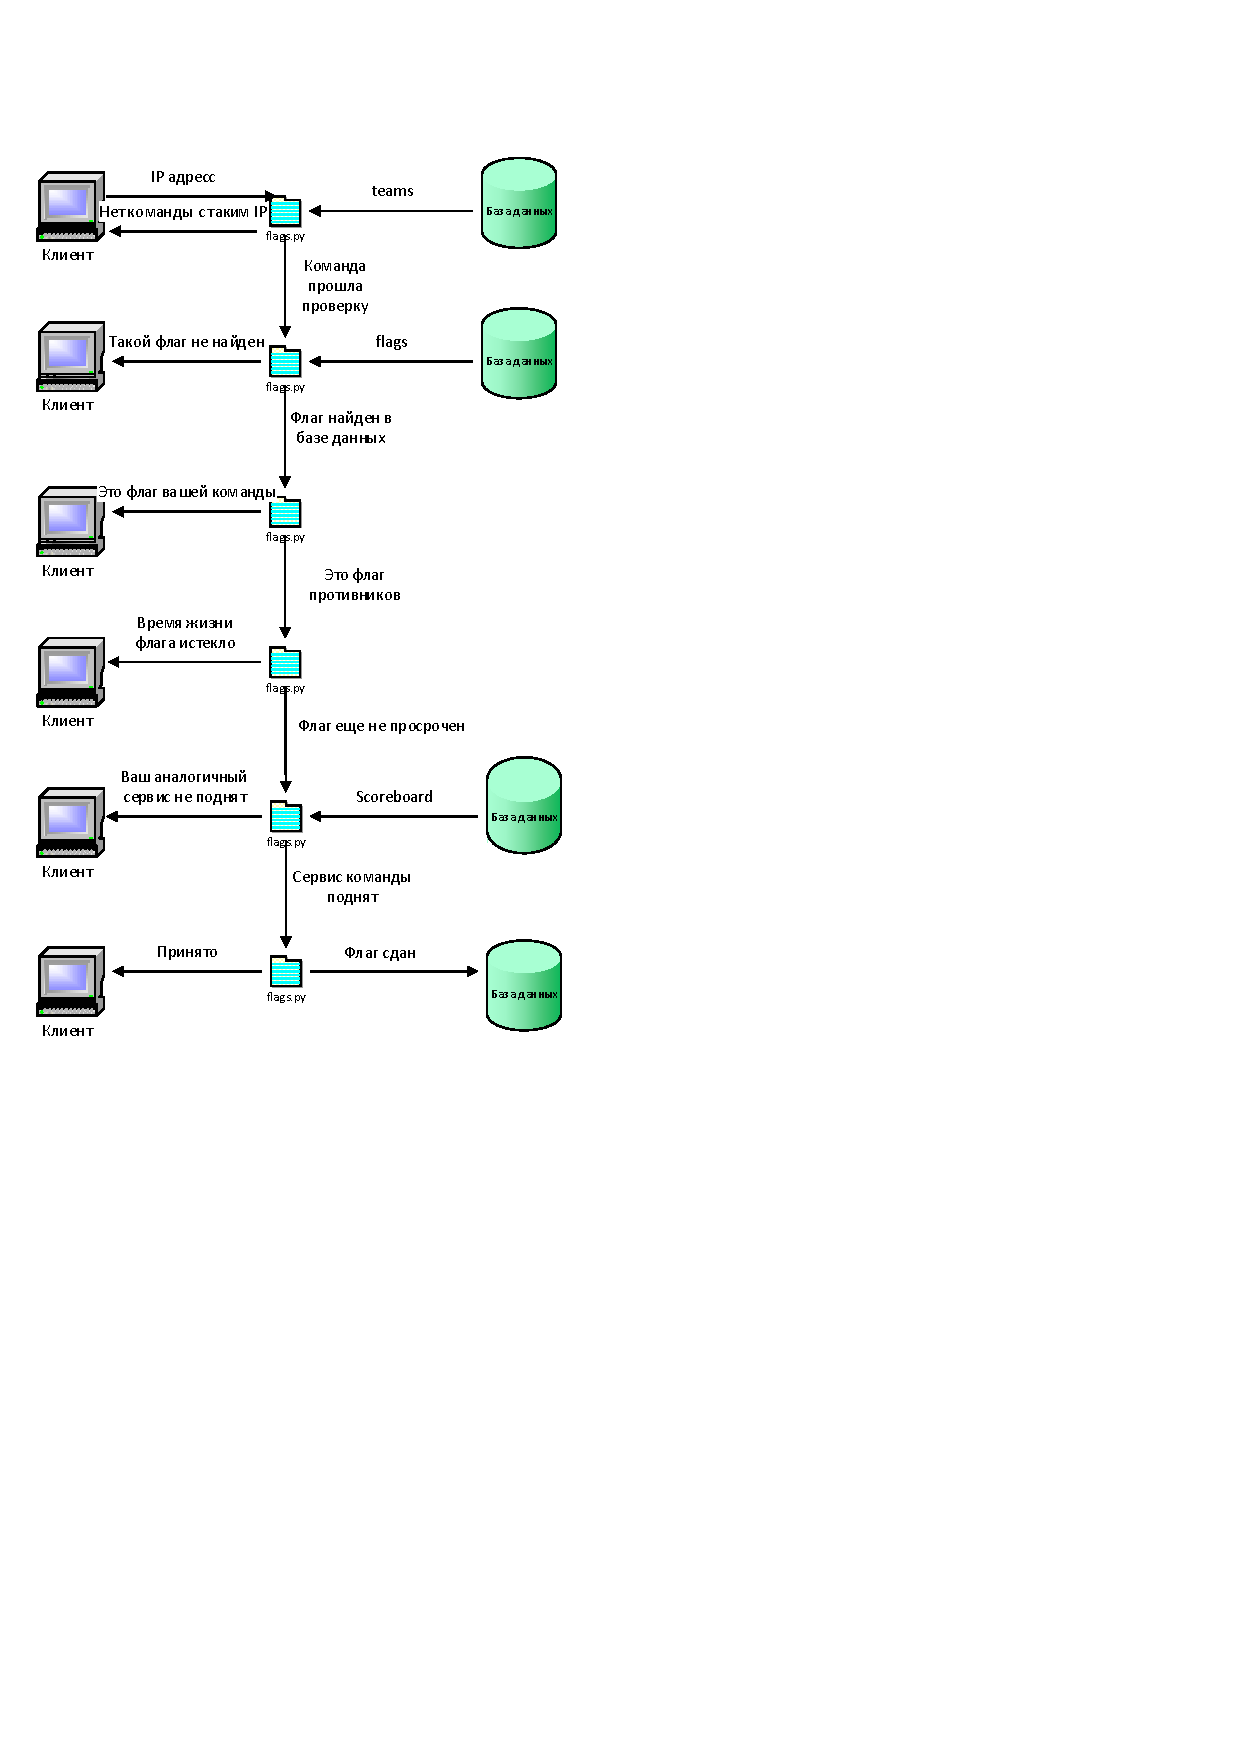
\includegraphics[trim=0 300 300 0, width=0.7\linewidth]{individual_reports/Naglyadno.pdf}}
\caption{Наглядная схема работы flags.py}
\end{figure} 

\clearpage


\subsection{Модуль: организации работы с сервисами} % - Отчёт round
Основное назначение платформы - общение с сервисами команд-участников посредством отправки и проверки специально сгенерированных флагов на сервере. Предназначение этого модуля - работа с интерфейсом сервисов (чекерами).

\subsubsection{Принцип работы}
Игра делится на раунды, каждый раунд, обычно, длится 1 минуту (настраивается при инициализации). Интерфейс для работы модуля с сервисом называется чекер. За этот период модуль опрашивает с помощью чекеров все сервисы команд-участников. Структура взаимодействия модуля с сервисами представлена на рисунке 5.4.

\begin{figure}[ht!]
\center{\includegraphics[width=1.0\linewidth]{images/module_round_structure.png}}
\caption{Иерархическая структура взаимодействия модуля с сервисами}
\end{figure}

Опрос происходит в три этапа:
\begin{enumerate} 
\item Проверка работоспособности сервиса команды-участника;
\item Отправление флага на сервис; 
\item Проверка того, что флаг сохранен.
\end{enumerate}

На каждом этапе модуль ожидает в ответ один из четырех чисел: 101, 102, 103, 104. Эти числа также называются статусом сервиса команды-участника. Алгоритм работы представлен на рисунке 5.5.

\begin{figure}[ht!]
\center{\includegraphics[width=0.5\linewidth]{images/module_round_schema.png}}
\caption{Схема создания потоков}
\end{figure}


Число 101 соответствует успешной работе сервиса команды-участника. Число 102 означает, что сервис команды работает, но на каком-то этапе отвечает некорректно. Число 103 означает, сервис команды отвечает, но не работает из-за какой-либо ошибки. Число 104 означает, что сервис команды не отвечает на запрос. 

Если на каком-то этапе чекер возвращает число отличное от 101, дальнейшее выполнение программы прекращается, а статус чекера записывается в базу данных.

На 1 этапе каждому чекеру посылается адрес сервера команды-участника. 
На 2 этапе каждому чекеру посылается адрес сервера, идентификатор флага и сам флаг. 
На 3 этапе каждому чекеру посылается адрес сервера, идентификатор флага и сам флаг.

Алгоритм работы представлен на рисунке 5.6.
\begin{figure}[ht!]
\center{\includegraphics[width=0.3\linewidth]{images/module_round_toservice.png}}
\caption{Блок-схема работы с каждым сервисом каждой команды-участника}
\end{figure}


Для увеличения производительности, каждый опрос сервисов команд-участников помещается в новый поток. Это позволяет работать в асинхронном режиме. Поэтому нестабильная работа сервиса команды-участника или ошибка в работе чекера не повлияет на опрос других сервисов. Также каждому потоку задается ограничение по времени работы. Это позволяет своевременно завершать процессы, тем самым уменьшается нагрузка на процессор и на потребление памяти.



\clearpage

\newpage
\section{Планы на будущее}
\begin{enumerate}
\item Составление руководств пользователя и администратора;
\item Проведение соревнований SibirCTF2016;
\item Привлечение к использованию данного программного комплекса, рекламируя продукт.
\end{enumerate}

\newpage
\section*{Заключение}
\addcontentsline{toc}{section}{Заключение}
В данном семестре нашей группой была выполнена часть работы по созданию платформы для проведения соревнований в области информационной безопасности, определены основные векторы развития и поставлены задачи для дальнейшего развития платформы.
 
 
 \newpage
 % \renewcommand{\refname}{Список использованных источников}
 \bibliography{lit}

 \ESKDappendix{Обязательное}{\normalfont Компакт-диск}
 Компакт-диск содержит: 
 \begin{itemize}
 \item электронную версию пояснительной записки в форматах *.tex и *.pdf;
 \item актуальную версию программного комплекса для проведения компьютерной экспертизы;
 \item тестовые данные для работы с программным комплексом;
 \item документацию к проекту в html-формате.
 \end{itemize}
 
\end{document}
